% ============================================================


\section{问题分析}

在展开具体建模之前，先明确本文所研究微网整体结构及主要能量流关系，如图\ref{fig:relationship}。


\begin{figure}[H]
  \centering
  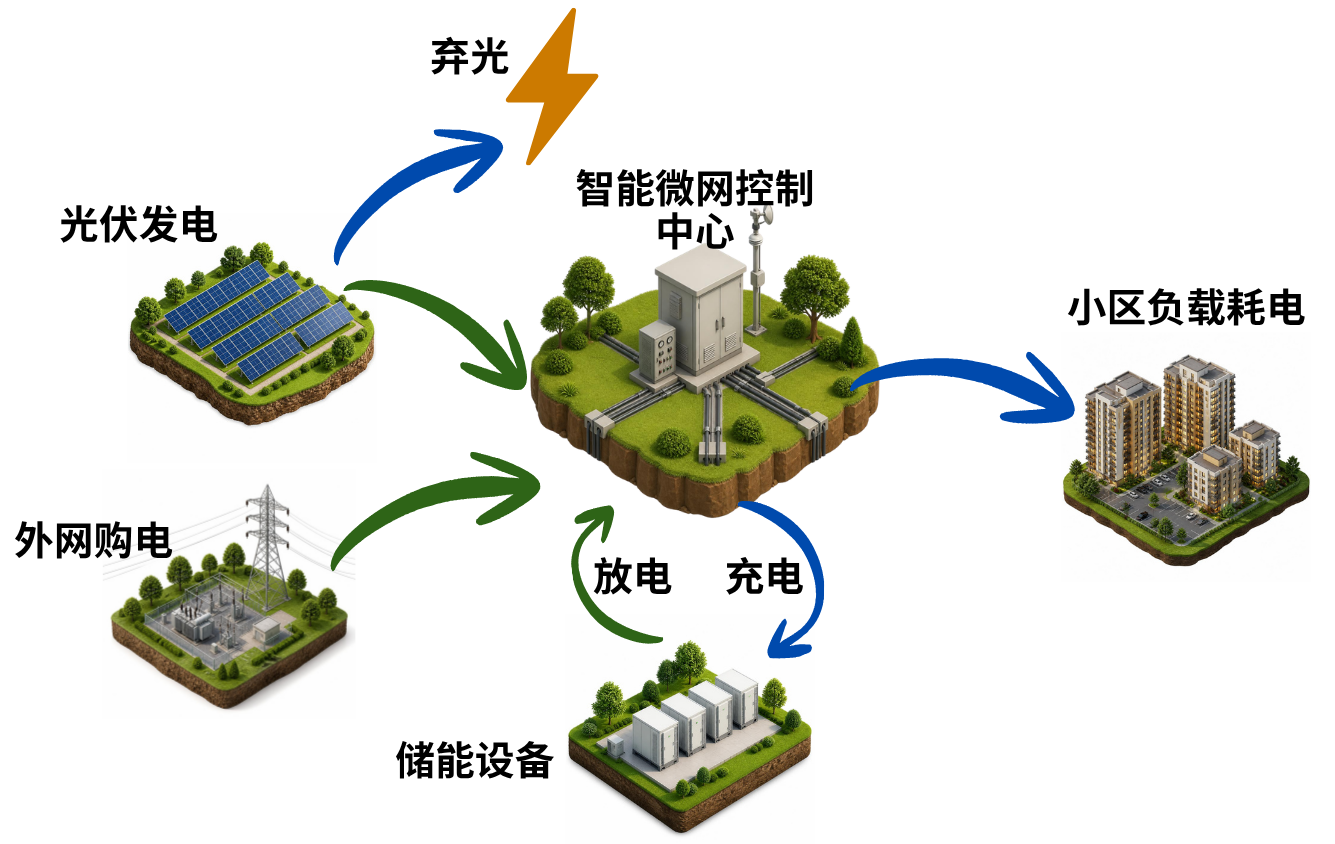
\includegraphics[width=0.70\linewidth]{figures/relationship.png}
  \caption{微网系统中光伏、外网、储能与小区负载间的能量流关系}
  \label{fig:relationship}
\end{figure}

控制中心统一调度光伏、外网购电两路输入及储能充放电，供给小区负荷；后续各问均围绕这一能量流展开，差异体现在决策时点、信息可得性与约束条件上。本文由确定性调度出发，逐步考虑预测不确定性、日内滚动调整及动态电价下的跨日决策，形成如下总体研究思路：

\begin{figure}[H]
  \centering
  \includegraphics[width=0.85\linewidth]{figures/our_work.png}
  \caption{总体研究思路流程图}
  \label{fig:overall-flow}
\end{figure}
